%\documentclass[tikz]{standalone}
\documentclass{article} % say
\usepackage{tikz}
\usepackage{courier}
\usetikzlibrary{arrows,decorations.pathmorphing,backgrounds,positioning,fit,petri}
\usetikzlibrary{shapes.multipart}
\begin{document}

\definecolor{pilosa-lightblue}{HTML}{E4EFF4}
\definecolor{pilosa-blue}{HTML}{3C5F8D}
\definecolor{pilosa-green}{HTML}{1DB598}
\definecolor{pilosa-red}{HTML}{ff2B2B}


logging output flow \\

upper section (blue+gray) describes flow from CLI flag to server. lower section
(red) describes how log output is ``inherited'' between objects, starting with the server\\

\\

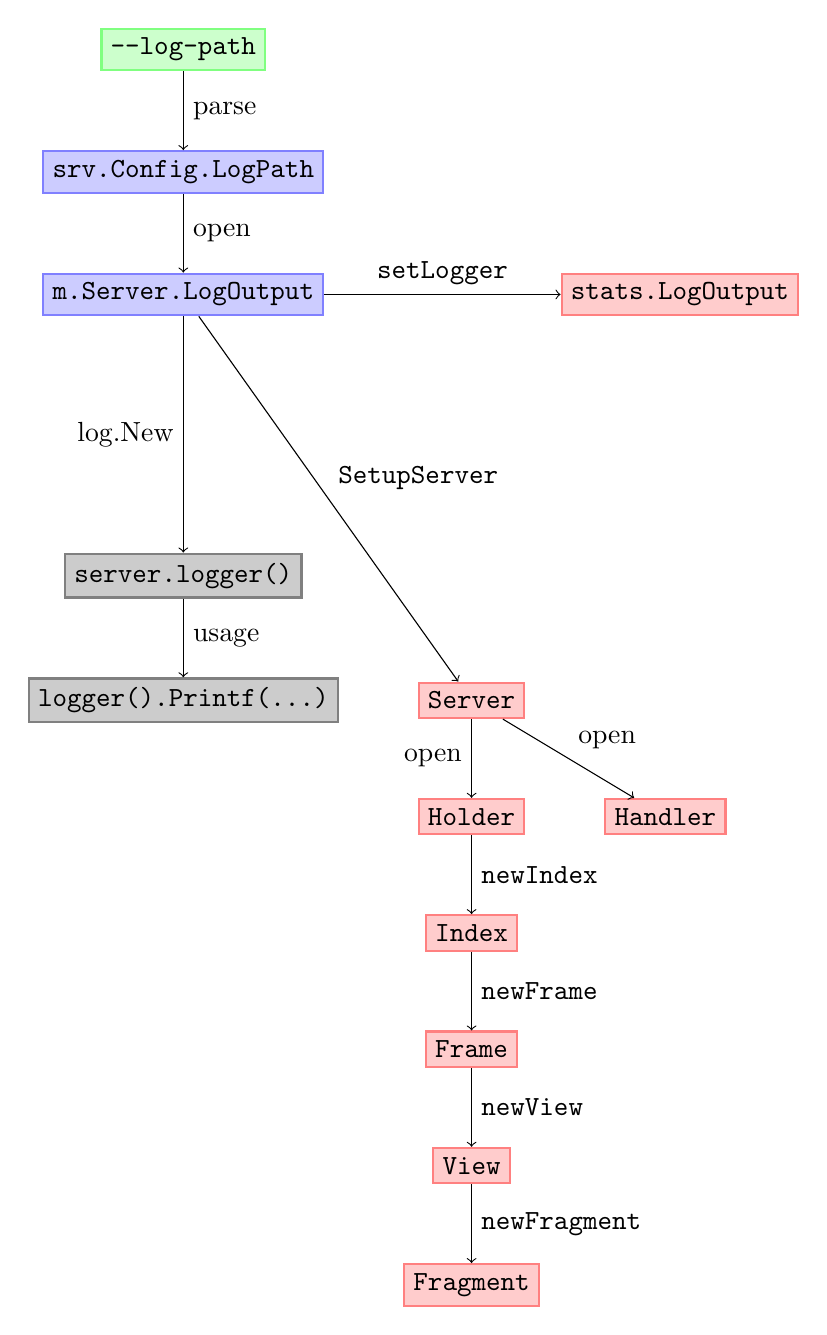
\begin{tikzpicture}
  [auto,
  flag/.style={rectangle,draw=green!50,fill=green!20,thick},
var/.style={rectangle,draw=blue!50,fill=blue!20,thick},
func/.style={rectangle,draw=black!50,fill=black!20,thick},
object/.style={rectangle,draw=red!50,fill=red!20,thick}]

% control flow
\node[flag] (logpath) {\texttt{--log-path}};  % CLI, ctl/server.go
\node[var] (config-logpath) [below=of logpath] {\texttt{srv.Config.LogPath}};  % server/server.go, setupServer
\node[var] (server-logoutput) [below=of config-logpath] {\texttt{m.Server.LogOutput}};  % server/server.go, setupServer
\node[func] (server-logger) [below=of server-logoutput,yshift=-2cm] {\texttt{server.logger()}};  % server.go
\node[func] (logger-print) [below=of server-logger] {\texttt{logger().Printf(...)}};  % several locations

\draw [->] (logpath) -- node [midway] {parse} (config-logpath) ;
\draw [->] (config-logpath) -- node [midway] {open} (server-logoutput);
\draw [->] (server-logoutput) -- node [swap,midway] {log.New} (server-logger);
\draw [->] (server-logger) -- node [midway] {usage} (logger-print);


% log output
\node[object] (stats) [right=of server-logoutput,xshift=2cm] {\texttt{stats.LogOutput}};

\node[object] (server) [right=of logger-print] {\texttt{Server}};
\node[object] (holder) [below=of server] {\texttt{Holder}};
\node[object] (handler) [below right=of server] {\texttt{Handler}};
\node[object] (index) [below=of holder] {\texttt{Index}};
\node[object] (frame) [below=of index] {\texttt{Frame}};
\node[object] (view) [below=of frame] {\texttt{View}};
\node[object] (fragment) [below=of view] {\texttt{Fragment}};

\draw [->] (server) -- node [swap,midway] {open} (holder) ;
\draw [->] (server) -- node [midway] {open} (handler) ;
\draw [->] (holder) -- node [midway] {\texttt{newIndex}} (index) ;
\draw [->] (index) -- node [midway] {\texttt{newFrame}} (frame) ;
\draw [->] (frame) -- node [midway] {\texttt{newView}} (view) ;
\draw [->] (view) -- node [midway] {\texttt{newFragment}} (fragment) ;


% connections from control flow to log output
\draw [->] (server-logoutput) -- node [midway] {\texttt{SetupServer}} (server);
\draw [->] (server-logoutput) -- node [midway] {\texttt{setLogger}} (stats);

\end{tikzpicture}
\end{document}
